\documentclass{article}
\usepackage[margin=2cm]{geometry}
\usepackage{polski}
\usepackage{amsmath}
\usepackage{graphicx}
\usepackage{svg}

\title{Technologie sieciowe \\ sprawozdanie 2}
\author{Krzysztof Nowak}

\begin{document}
    \maketitle

    \section{Badany model sieci}
    Badana sieć komputerowa została przedstawiona na rysunku \ref{fig:graph}. Została narysowana ręcznie. Posiada 20 węzłów i 29 krawędzi. Macierz natężeń o wymiarze 20x20 została wygenerowana losowo, przyjmuje wartości z zakresu $(30; 100)$, wartości na przekątnej wynoszą 0.  Założono, że pakiety poruszają się najkrótszą (pod względem liczby krawędzi) ścieżką między nadawcą, a odbiorcą. Ścieżka ta była wyznaczana przy pomocy algorytmu Dijkstry. Przepustowość krawędzi została określona jako $c(e) = 2a_0(e)$, gdzie $a_0(e)$ oznacz liczbę pakietów na sekundę przesyłanych przez połączenie $e$ w pełni sprawnej sieci.

    \begin{figure}[h]
        \centering
        \includegraphics[width=12cm]{../network.png}
        \caption{Graf reprezentujący połączenia w sieci}
        \label{fig:graph}
    \end{figure}


    % \begin{table}
    %     \caption{Macierz natężeń, liczba pakietów na sekundę pomiędzy poszczególnymi węzłami.}
    %     \label{tab:macierz}
    % \end{table}

    \section{Metoda badań}
    Zachowanie sieci badane jest poprzez 1000 krotne uruchomieni symulacji dla zadanych wartości parametrów. Przy każdym uruchomieniu losowo z prawdopodopieństwem $(1-p)$ z sieci usuwane są połączenia, a następnie sprawdzane są następujące warunki:
    \begin{itemize}
        \item spójność grafu,
        \item obciążenie poszczególnych połączeń - $\left(\forall e\right)\left(c(e) \geq a(e)\right)$,
        \item średie opóźnienie $T = \cfrac{1}{G} \sum_{e \in E} \cfrac{a(e)}{c(e) - a(e)} < T_{max}$.
    \end{itemize}

    Gdy dany warunek nie jest spełniony, zostaje to odnotowane, a kolejne nie są sprawdzane. Za maksymalne opóźnienie $T_{max}$ przyjęto $1.1 T_0$, gdzie $T_0$ oznacza średni czas opóźnienia w pełni sprawnej sieci.


    \section{Wpływ niezawodności $p$ na funkcjonowanie sieci}
    W pierszym eksperymencie badano wpływ wartości $p$, która opisuje prawdopodopieństwo prawidłowego działania jednej krawędzi, na poprawne funkcjonowanie sieci. Wyniki przedstawiono na wykresie \ref{fig:exp_p2}. Gdy $p=1.0$, cała sieć również jest sprawna. Gdy niezawodność $p$ jest niska, $p<0.75$, dominującym problemem staje się niespójność sieci. 
    \begin{figure}[h]
        \centering
        \includegraphics[width=12cm]{../experiment_p2.png}
        \label{fig:exp_p2}
        \caption{Wpływ niezawodności pojedynczych połączeń na niezawodność sieci, $p\in<0.0;1.0>$}
    \end{figure}

    Tak wysoka awaryjność zdje się nie odzwierciedlać rzeczywistości, dlatego skupiono się na przedziale $p \in <0.9; 1.0>$. Wyniki przedstawiono na \ref{fig:exp_p}. Obserwujemy, że wraz ze spadkiem $p$ częstsze stają się przekroczenia limity obciążeń pojedynczych krawędzi. Przkroczenia czasu opóźnienia zdarzają się względnie rzadko, prawdopodobnie dlatego, że przyjęto duży (dwukrotny) zapas przepustowości, każdego połączenia. 


    \begin{figure}[h]
        \centering
        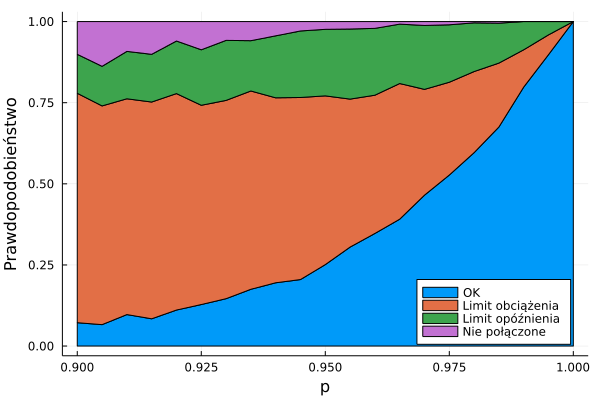
\includegraphics[width=12cm]{../experiment_p.png}
        \label{fig:exp_p}
        \caption{Wpływ niezawodności pojedynczych połączeń na niezawodność sieci, $p\in<0.9;1.0>$}
    \end{figure}

    Dla $p=0.975$ zachowanie sieci jest najbardziej zróżnicowane, dlatego ta wartość zostanie przyjęta dla dalszych eksperymentów.

    \newpage
    \section{Wpływ intensywności ruchu na niezawodność sieci}
    W kolejnym eksperymencie badano jak wzrost intensywności ruchu ma wpływ na sieć. W tym celu, każdy element macierzy $N$ został przemnożony przez $k <0.1; 10>$. Wyniki przedstawiono na wykresie \ref{fig:exp_n}. Wzrost intensywności najpierw powoduje wzrost częstotliwości przekroczenia maksymalnego opóźnienia, a przy większych przeciążenia, doprowadza do saturacji poszczególnych połączeń. Z kolei zmniejszanie zadanego ruchu sieciowego, zmniejsza występowanie przkroczeń limitów.

    \begin{figure}[h]
        \centering
        \includegraphics[width=12cm]{../experiment_N.png}
        \label{fig:exp_n}
        \caption{Zależność między intensywnością ruchu, a niezawodnością sieci}
    \end{figure}

    \section{Wpływ zmiany topologi sieci na jej niezawodność}
    W ostatnim eksperymencie badano, jak dodawanie nowych połączeń wpływa na niezawodność sieci. Do grafu dodawano krawędzi łączące losowe wierzchołki, dopóki liczba krawędzi $e$ nie osiągneła żądnaej wartości. Dla każdego $e$ generowano nowe połączenia na 30 sposobów, a dla każdego z nich przeprowadzono 100 testów awaryjność. Badano $e \in <29; 100>$. Wyniki przedstawiono na wykresie \ref{fig:exp_topo}. Wzrost liczby połączeń zwiększa niezawodność sieci.

    \begin{figure}[h]
        \centering
        \includegraphics[width=12cm]{../experiment_topo.png}
        \label{fig:exp_topo}
        \caption{Zależność między liczbą połączeń, a niezawodnością}
    \end{figure}


\end{document}